%-----------------------------------------
% Note: Use pdflatex to process this file.
%-----------------------------------------

%\documentclass{report}
\documentclass{hitec}

\usepackage{setspace}
\usepackage{graphicx}
\usepackage{moreverb}    % Defines {listing} environment.
\usepackage{amsmath, amsthm, amssymb, amsbsy, mathtools}
\usepackage{alltt}
\usepackage{rotating}
\usepackage[TABBOTCAP]{subfigure}
\usepackage{toc-bmad}
\usepackage{xspace}
%%\usepackage{makeidx}
\usepackage[section]{placeins}   % For preventing floats from floating to end of chapter.
\usepackage{longtable}  % For splitting long vertical tables into pieces
\usepackage{index}
\usepackage{multirow}
\usepackage{booktabs}   % For table layouts
\usepackage{yhmath}     % For widehat

\usepackage[T1]{fontenc}   % so _, <, and > print correctly in text.
\usepackage[strings]{underscore}    % to use "_" in text
\usepackage[pdftex,colorlinks=true]{hyperref}   % Must be last package!

%----------------------------------------------------------------

\newcommand{\extref}[1]{$\S$\ref*{#1}}   % No hyperlink. For external refs. \extref
\newcommand{\comma}{\> ,}
\newcommand{\period}{\> .}
\newcommand{\wt}{\widetilde}
\newcommand{\grv}{\textasciigrave}
\newcommand{\hyperbf}[1]{\textbf{\hyperpage{#1}}}
\newcommand{\Ss}{\(^*\)}
\newcommand{\Dd}{\(^\dagger\)}

\newcommand{\AND}{&& \hskip -17pt\relax}
\newcommand{\CR}{\\}
\newcommand{\CRNO}{\nonumber \\}
\newcommand{\dstyle}{\displaystyle}

\newcommand{\Begineq}{\begin{equation}}
\newcommand{\Endeq}{\end{equation}}
\newcommand{\NoPrint}[1]{}

\newcommand{\pow}[1]{\cdot 10^{#1}}
\newcommand{\Bf}[1]{{\bf #1}}
\newcommand{\bfr}{\Bf r}

\newcommand{\bmad}{{\sl Bmad}\xspace}
\newcommand{\tao}{{\sl Tao}\xspace}
\newcommand{\mad}{{\sl MAD}\xspace}
\newcommand{\cesr}{{\sl CESR}\xspace}

\newcommand{\sref}[1]{\S\ref{#1}}
\newcommand{\Sref}[1]{Sec.~\sref{#1}}
\newcommand{\cref}[1]{Chapter~\ref{#1}}

\newcommand{\Newline}{\hfil \\ \relax}

\newcommand{\eq}[1]{{(\protect\ref{#1})}}
\newcommand{\Eq}[1]{{Eq.~(\protect\ref{#1})}}
\newcommand{\Eqs}[1]{{Eqs.~(\protect\ref{#1})}}

\newcommand{\vn}{\ttcmd}           % For variable names
\newcommand{\vni}{\ttcmdindx}
\newcommand{\cs}{\ttcmd}           % For code source
\newcommand{\cmd}{\ttcmd}          % For Unix commands
\newcommand{\rn}{\ttcmd}           % For Routine names
\newcommand{\tn}{\ttcmd}           % For Type (structure) names
\newcommand{\bn}[1]{{\bf #1}}       
\newcommand{\toffset}{\vskip 0.01in}
\newcommand{\rot}[1]{\begin{rotate}{-45}#1\end{rotate}}

\newcommand{\data}{{\mbox{data}}}
\newcommand{\reference}{{\mbox{ref}}}
\newcommand{\model}{{\mbox{model}}}
\newcommand{\base}{{\mbox{base}}}
\newcommand{\design}{{\mbox{design}}}
\newcommand{\meas}{{\mbox{meas}}}
\newcommand{\var}{{\mbox{var}}}

\newcommand\ttcmd{\begingroup\catcode`\_=11 \catcode`\%=11 \dottcmd}
\newcommand\dottcmd[1]{\texttt{#1}\endgroup}

\newcommand\ttcmdindx{\begingroup\catcode`\_=11 \catcode`\%=11 \dottcmdindx}
\newcommand\dottcmdindx[1]{\texttt{#1}\endgroup\index{#1}}

\newcommand{\St}{$^{st}$\xspace}
\newcommand{\Nd}{$^{nd}$\xspace}
\newcommand{\Th}{$^{th}$\xspace}
\newcommand{\B}{$\backslash$}
\newcommand{\W}{$^\wedge$}

\newcommand{\cbar}[1]{\overline C_{#1}}

\newlength{\dPar}
\setlength{\dPar}{1.5ex}

\newenvironment{example}
  {\vspace{-3.0ex} \begin{alltt}}
  {\end{alltt} \vspace{-2.5ex}}

\newcommand\Strut{\rule[-2ex]{0mm}{6ex}}

\newenvironment{Itemize}
  {\begin{list}{$\bullet$}
    {\addtolength{\topsep}{-1.5ex} 
     \addtolength{\itemsep}{-1ex}
    }
  }
  {\end{list} \vspace*{1ex}}

\newcommand{\Section}[1]{\section{#1}\indent\vspace{-3ex}}

\newcommand{\SECTION}[1]{\section*{#1}\indent\vspace{-3ex}}

% From pg 64 of The LaTex Companion.

\newenvironment{ventry}[1]
  {\begin{list}{}
    {\renewcommand{\makelabel}[1]{\textsf{##1}\hfil}
     \settowidth{\labelwidth}{\textsf{#1}}
     \addtolength{\itemsep}{-1.5ex}
     \addtolength{\topsep}{-1.0ex} 
     \setlength{\leftmargin}{5em}
    }
  }
  {\end{list}}


\renewcommand{\ttdefault}{txtt}

\renewcommand{\textfraction}{0.1}
\renewcommand{\topfraction}{1.0}
\renewcommand{\bottomfraction}{1.0}

\settextfraction{0.9}

\title{Quick Introduction to Accelerator \& X-Ray \\ Simulations Using Bmad and Tao}
\author{}
\date{David Sagan \\ June 21, 2016}
\begin{document}
\maketitle

%------------------------------------------------------------------------------
\section{Overview}

First off, let's define some terms:
  \begin{description}
  \item[Bmad] \Newline
\bmad is an open-source software library (aka toolkit) for simulating charged particles
and X-rays. \bmad is not a program itself but is used by programs for doing
calculations. 
  \item[Tao] \Newline
\tao is a general purpose simulation program, based upon \bmad. \tao can be used to
view lattices, design lattices, track particles through lattices, etc.
  \end{description}

%------------------------------------------------------------------------------
\section{Resources}

More information is readily available at the \bmad and \tao web site:
\begin{alltt}
  \url{http://www.lepp.cornell.edu/~dcs/bmad}
\end{alltt}
Links to the \bmad and \tao manuals can be found there as well as instructions for
downloading and setup.

%------------------------------------------------------------------------------
\section{What Can Bmad Do?}

Over the years, \bmad has been used for a wide range of charged-particle and X-ray
simulations. The following list gives some idea as to the range that \bmad has been put to use
for:
\begin{alltt}
  Lattice design                              X-ray simulations
  Spin tracking                               Wakefields and HOMs
  Beam breakup simulations in ERLs            Touschek Simulations
  Intra-beam scattering (IBS) simulations     Dark current tracking
  Coherent Synchrotron Radiation (CSR)        Frequency map analysis
\end{alltt}


%------------------------------------------------------------------------------
\section{Orientation}

  \begin{description}
  \item[Distributions and Releases] \Newline
A \vn{Release} is a build of \bmad and associated libraries and programs (including \tao)
that is done on the Linux computer system at CLASSE (Cornell's Laboratory for
Accelerator-based Sciences and Education). A \vn{Distribution} is like a \vn{Release},
except it is done outside of the CLASSE Linux computer system.  For the purpose
of this introduction, \vn{Releases} and \vn{Distributions} are considered to be the same.
  \end{description}

It is assumed that you already of access to a \vn{Distribution} or a \vn{Release} and that
you have setup the requisite environmental variables. If this is not true, and there is no
local Guru to gide you, download and setup instructions can be found on the \bmad web
site. If everything is setup correctly, the environmental variable \vn{ACC_ROOT_DIR} will
point to the root directory of the Distribution or Release you are using. For a
Distribution, this directory looks something like:
\begin{alltt}
  ~> ls \$ACC_ROOT_DIR

  PGPLOT                debug       h5hut        plplot                tao
  bmad                  examples    hdf5         production            util
  bsim                  fgsl        include      recipes_f-90_LEPP     util_programs
  build_system          forest      lapack       regression_tests      xraylib
  cpp_bmad_interface    gsl         lattice      sim_utils             xsif
\end{alltt}

For an expanation of what directories contain what, see:
\begin{alltt}
  \url{https://wiki.classe.cornell.edu/ACC/ACL/OffsiteDoc#DistDirs}
\end{alltt}

A quick introduction to the most important directories:
  \begin{description}
  \item[bmad] \Newline
The \vn{bmad} directory holds the code for the \bmad library.
  \item[bsim] \Newline
The \vn{bsim} directory holds some \bmad based simulation programs for simulating
synchrotron radiation (programs: \vn{synrad} and \vn{synrad3d}), dynamic_aperture
(program: \vn{dynamic_aperture}), intra beam scattering (programs: \vn{ibs_linac} and
\vn{ibs_ring}), etc.
  \item[examples] \Newline
The \vn{alltts} directory holds example programs along with example lattice files.
  \item[production] \Newline
The \vn{production/bin} directory contains executable files for \tao, etc. [This
directory is created in a \vn{distribution} when the \bmad code is compiled.]
  \item[tao] \Newline
The \vn{tao} directory holds the code for the \tao program as well as example input
files.
  \end{description}

%------------------------------------------------------------------------------
\section{The Lattice}

The first thing you will need when working with \bmad is a \bmad compatable lattice file.
If you have a file suitable for MAD-8, MAD-X, or SAD, these can be translated to \bmad
format. 

For MAD-8 or MAD-X, the translator is via the Accelerator Markup Language /
Universal Accelerator Parser Project. Details about AML/UAP are at:
\begin{alltt}
  \url{http://www.lepp.cornell.edu/~dcs/aml/}
\end{alltt}

For translation from SAD, there is a python script for this at:
\begin{alltt}
   \$ACC_ROOT_DIR/util_programs/sad_to_bmad/
\end{alltt}

If you want to create a \bmad lattice from scratch, documentation is in the \bmad manual
in the \vn{Language Reference} section. Also look at the examples in:
\begin{alltt}
  \$ACC_ROOT_DIR/examples/lattice_file_examples
  \$ACC_ROOT_DIR/lattice           # Cornell centric lattices
\end{alltt}

Here is a very simple example just to illustrate what a lattice file looks
like. Everything here is explained in much more detail in the \bmad manual
\begin{alltt}
  parameter[geometry] = open     ! open geometry => Linac, transfer line, etc.
  parameter[e_tot] = 1e6         ! Reference particle total energy (eV).
  beginning[beta_a] = 10         ! Horizontal mode starting Twiss parameter.
  beginning[beta_b] = 20         ! Vertical mode starting Twiss parameter.

  q1: quadrupole, l = 1, k1 = 0.6   ! Define a quadrupole element
  lc: lcavity, l = 2, voltage = 1e7 ! Define an accelerating cavity.
  my_line: line = (q1, lc)          ! ordered list of elements to track through.
  use, my_line                      ! The line to be used.
\end{alltt}
This example creates a lattice with two elements named \vn{q1} AND \vn{lc}

%------------------------------------------------------------------------------
\section{Using Tao to Examine Lattices}

%------------------------------------------------------------------------------
\subsection{Starting Tao}

The \tao program is useful for examining lattices. As an example, run \tao with
the following command
\begin{alltt}
  \$ACC_ROOT_DIR/production/bin/tao -noinit -lat \B
              \$ACC_ROOT_DIR/tao/examples/cesr/bmad_L9A18A000-_MOVEREC.lat
\end{alltt}
The \vn{-noinit} option prevents a \tao initialization file from being read in (more
on this later). The \vn{-lat} option is used to specify a lattice file. In this case,
a lattice file for Cornell's Cesr ring is used. For a list of options when starting
up \tao see the \tao manual or start \tao with the command:
\begin{alltt}
  \$ACC_ROOT_DIR/production/bin/tao -help
\end{alltt}

After \tao is started, commands may be entered on the command line. The section
\tao \vn{Line Mode Commands} in the \tao manual lists the possible commands. The list
of commands may also be viewd by typing \vn{help} on the command line:
\begin{alltt}
  {\normalfont\textbf{Tao> help}}

  Type 'help <command>' for help on an individual command
  Available commands:
    alias                             read
    call                              restore
    change                            reinitialize
    clip                              run_optimizer
    continue                          scale
    derivative                        set
    end_file                          show
    exit                              single_mode
    flatten                           spawn
    help                              timer
    history                           use
    misalign                          veto
    pause                             value
    place                             wave
    plot                              write
    ptc                               x_axis
    python                            x_scale
    quit                              xy_scale
\end{alltt}

%------------------------------------------------------------------------------
\subsection{Tao Plotting}

\begin{figure}[t]
\begin{centering}
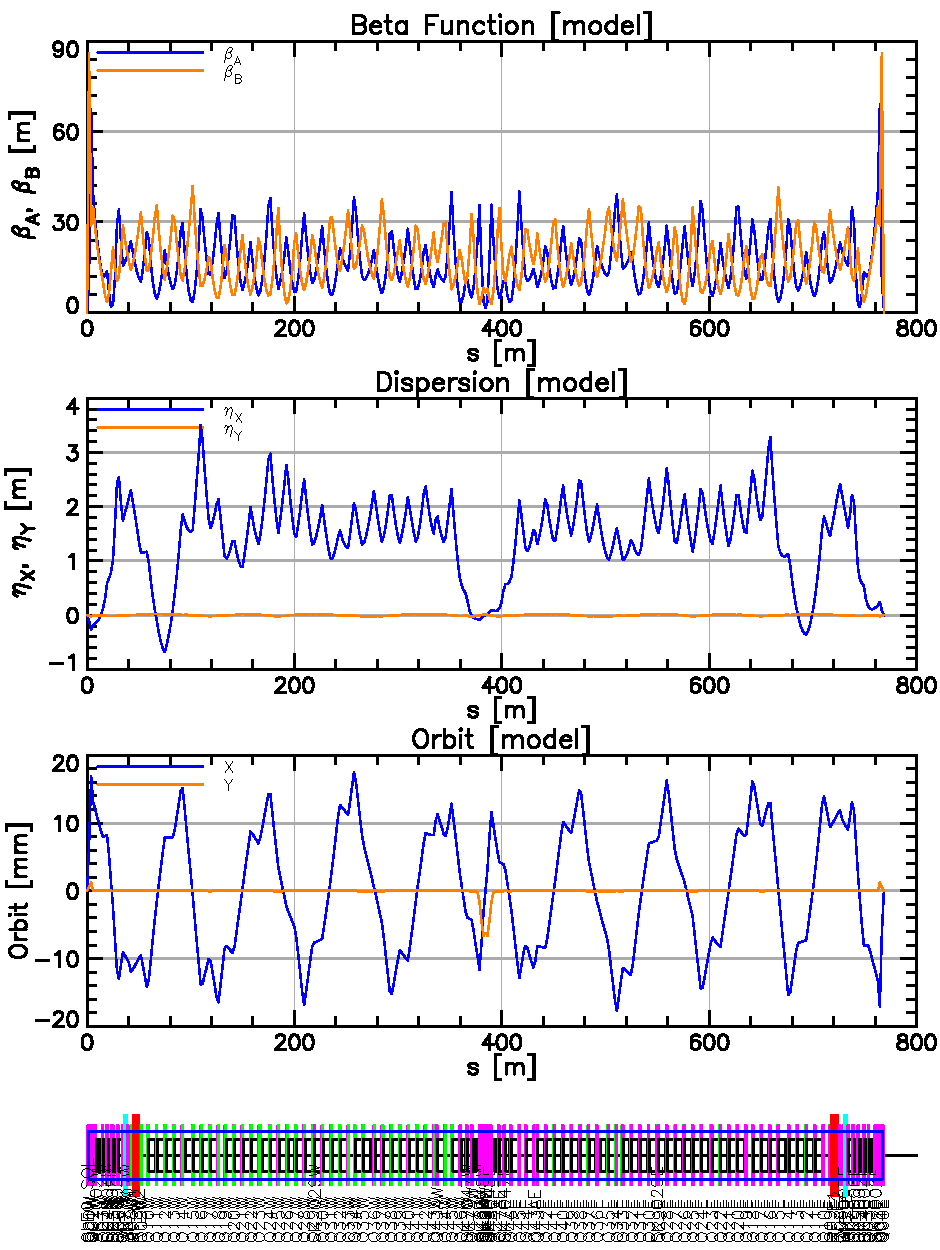
\includegraphics[width=3in]{tao-start.pdf}
\hfill
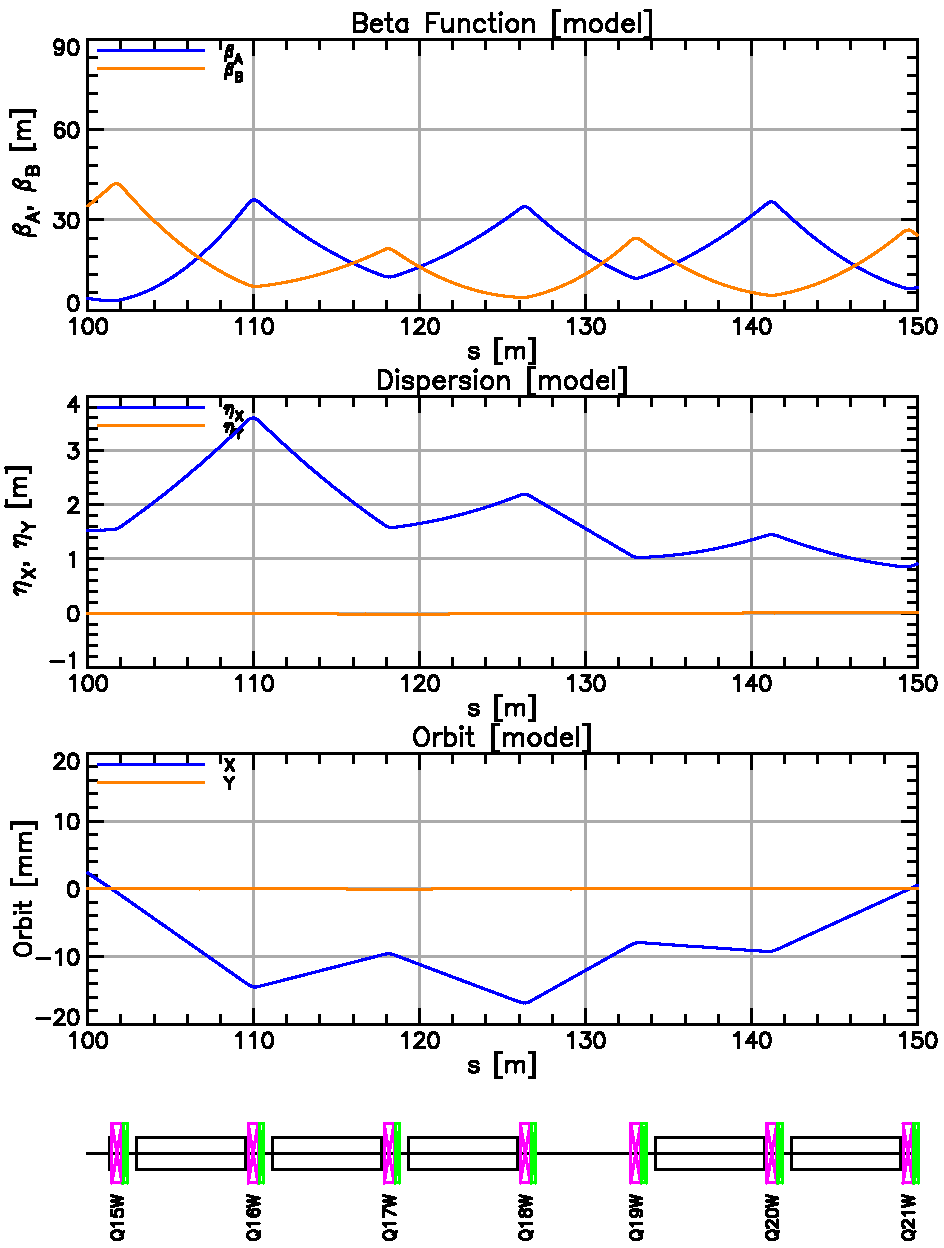
\includegraphics[width=3in]{tao-x-scale.pdf}
\caption{Left: Initial \tao plot window with the bmad_L9A18A000-_MOVEREC.lat lattice.
Right: Plot window after horizontal scaling.}
\label{f:tao-start}
\end{centering}
\end{figure}

If all goes well, \tao will pop up a plotting window as shown on the left in
\fig{f:tao-start}. If the plot window is too small or two large, the \vn{-geometry} option
can be used at startup to specify the window size. For example:
\begin{alltt}
  \$ACC_ROOT_DIR/production/bin/tao -geometry 300x500 -lat ....
\end{alltt}
With this example, \tao would open a plotting window 300 pixels wide by 500 pixels tall.
To prevent any plotting, use the \vn{-noplot} option.

The plot can be scalled vertically using the \vn{scale} command. To scale the plot horizontally, 
the command \vn{x_scale} is used. Thus to scale all the plots horizontally in our present example use
\begin{alltt}
  Tao> x_sca all 100 150
\end{alltt}
This scales all the horizontal scale to go from 100~meters to 150~meters.  Notice that
commands can be abbreviated.

The \vn{show plot} command will give some details on plotting:
\begin{alltt}
  {\normalfont\textbf{Tao> show plot}}

    plot_page parameters:
    %size                         =      500     600
    %n_curve_pts                  =      401
    %text_height                  = 12.000
    %main_title_text_scale        = 1.300
    %graph_title_text_scale       = 1.100
    %axis_number_text_scale       = .900
    ... ETC., ETC ...

  Templates:
     Plot                  .Graph   Description
     --------------------  -------- -------------------
     alpha                 .g       Twiss alpha function
     b_div_curl            .g       Magnetic Field Divergence and Curl along orbit
     b_field               .g       Magnetic Field Along Orbit
     beta                  .g       Twiss beta function
     cbar                  .g       Cbar coupling matrix
     dbeta                 .g       Chromatic normalized beta beat
     deta                  .g       Second order dispersion
     detap                 .g       Second order dispersion slope
     dphi                  .g       Chromatic phase deviation
     dynamic_aperture      .g       Dynamic aperture using universe calc
     e_div_curl            .g       Electric Field Divergence and Curl along orbit
     e_field               .g       Electric Field Along Orbit
     emittance             .g       Linac emittance
     energy                .g       Particle energy
     dispersion            .g       X & Y Dispersion
     mode_dispersion       .g       A & B Normal Mode Dispersion
     floor_plan            .g1      Floor plan drawing of lattice elements.
    ... ETC., ETC ...

                                                 Location on Page
  Plot Region         <-->  Plot                 x1    x2    y1    y2
  -----------               -----------------------------------------
  layout              <-->  lat_layout          0.00  1.00  0.00  0.15
  r11                 <-->                      0.00  1.00  0.15  1.00
  r12                 <-->                      0.00  1.00  0.58  1.00
  r22                 <-->                      0.00  1.00  0.15  0.58
  r13                 <-->  beta                0.00  1.00  0.72  1.00
  r23                 <-->  dispersion          0.00  1.00  0.43  0.72
  r33                 <-->  orbit               0.00  1.00  0.15  0.43
    ... ETC., ETC ...
\end{alltt}
See the \vn{Plotting} chapter in the \tao manual as well as the \vn{Initializing
Plotting} section of the \vn{Tao Initialization} chapter. Essentially, the plot window is
divided into \vn{regions}. By default (without any initialization file), these regions
have names like \vn{r13}, \vn{r22}, etc. By default, the \vn{beta} plot, for example, is
placed in the \vn{r13} region and the \vn{r13} regions inhabits roughly the top of third
of the plot window. To change what plots are displayed, use the \vn{place} comand:
\begin{alltt}
  Tao> place r23 energy  ! Put an energy plot in the r23 region
\end{alltt}

%------------------------------------------------------------------------------
\subsection{Tao Initialization Files}



%------------------------------------------------------------------------------
\subsection{Examining Elements in Tao}

show universe

%------------------------------------------------------------------------------
\subsection{Changing Element Attributes in Tao}

%------------------------------------------------------------------------------
\subsection{Lattice Optimization in Tao}


%------------------------------------------------------------------------------
\subsection{Customizing Tao}

Besides the custimizaiton that can be done via \tao input files, \tao custom code
can be linked with \tao to extend \tao capabilities. For example, custom code can
be used to interface between \tao and an accelerator. In this way \tao can be used
as an online model to, for example, read orbit data, calculate via optimization corrector
strengths, and then load the calculated corrector changes back into the machine.

For more details on using custom code with \tao, see the \vn{Customizing Tao} chapter
in the \tao manual.

%------------------------------------------------------------------------------
\section{Creating Your Own programs}

At some point you might want to start creating you own programs. Documentation for this is
at:
\begin{alltt}
  \url{https://wiki.classe.cornell.edu/ACC/ACL/BuildSystem}
\end{alltt}

As a simple example, consider setting things up to compile the simple bmad program
discussed in the \vn{Introduction ot Bmad Programming} chapter of the \bmad manual.
The program code and lattice input file is in the directory:
\begin{alltt}
  \$ACC_ROOT_DIR/examples/simple_bmad_program/
\end{alltt}

The first thing to do is to create a \vn{base} directory for your code and executables. This
directory will be named \vn{base_dir} in this example but you can name it anything you
want. Important: Do not create \vn{base_dir} within a \vn{Distribution} tree. Keeping things
separate greatly simplifies maintainance.

After you have created \vn{base_dir}, cd to that directory. Now copy the
simple_bmad_program directory to a new directory called \vn{base_dir/my_prog_dir}:
\begin{alltt}
  base_dir> cp -r \$ACC_ROOT_DIR/examples/simple_bmad_program/ my_prog_dir
  base_dir> cd my_prog_dir
  my_prog_dir> ls

  lat.bmad   layout.bmad   simple_bmad_program.f90
\end{alltt}

The \vn{my_prog_dir} directory has the program code and lattice files but is
missing the \vn{cmake} scripts for compiling and linking the program.  [\vn{cmake} is the
open-source tool used to compile \bmad.] The scripts used by the \vn{Distribution} or
\vn{Release} for compiling are structured for a different directory organization so they
are not appropriate here. Rather, the ``template'' scripts in
examples/cmake_template_scripts work well so copy them into the my_prog_dir
directory:
\begin{alltt}
  my_prog_dir> cp \$ACC_ROOT_DIR/examples/cmake_template_scripts/* .
  my_prog_dir> ls

  CMakeLists.txt  cmake.test  lat.bmad  layout.bmad simple_bmad_program.f90
\end{alltt}

The scripts are setup to create an executable:
\begin{alltt}
  base_dir/production/bin/test
\end{alltt}
If you don't like the name \vn{test} then this can be changed by editing the
\vn{cmake.test} file and changing \vn{EXENAME}. In any case, to create the executable,
make sure you are still in the my_prog_dir directory and issue the \vn{mk} command:
\begin{alltt}
  my_prog_dir> mk
\end{alltt}

After the \vn{mk} command is finished there should be an executable at
\vn{base_dir/production/bin/test}. There will also be a \vn{my_prog_dir/production}
directory that holds intermediate compiled files which can be used in the future to save
compile time when there are multiple code files but not all of them have to be recompiled.
There is nothing in the \vn{my_prog_dir/production} of interest so it can be ignored.

Now you can run the program. While still in the \vn{my_prog_dir} directory (since the
program will look for the lattice file in the default directory), run the program:
\begin{alltt}
  ../production/bin/test
\end{alltt}
The result:
\begin{alltt}
  [INFO] bmad_parser:
      Parsing lattice file(s). This might take a minute or so...
  [INFO] bmad_parser:
      Created new digested file
    Ix  Name              Ele_type                   S      Beta_a
     0  BEGINNING         BEGINNING_ELE             0.0000      0.9379
     1  IP_L0             MARKER                    0.0000      0.9379
     2  CLEO_SOL#3        SOLENOID                  0.6223      1.3472
     3  DET_00W           MARKER                    0.6223      1.3472
     4  CLEO_SOL#4        SOLENOID                  0.6380      1.3682
     5  Q00W\\CLEO_SOL     SOL_QUAD                  1.7550      8.0285
     6  Q00W#1            QUADRUPOLE                2.1628     16.8607
     7  D003              DRIFT                     2.4934     28.5769
     8  DET_01W           MARKER                    2.4934     28.5769
     9  D004              DRIFT                     2.9240     48.4524
    10  Q01W              QUADRUPOLE                3.8740     66.8800
   
   !---------------------------------------------------------
   ! Information on element: CLEO_SOL
   
    Element #              872
    Element Name: CLEO_SOL
    Key: Solenoid
    S:              1.755000
    Ref_time:  5.854050E-09
   
    Attribute values [Only non-zero/non-default values shown]:
        1   L                            =  3.5100000E+00
        5   KS                           = -8.4023386E-02
       13   SPIN_FRINGE_ON               =  T (1)
       31   L_HARD_EDGE                  =  3.5100000E+00
       49   BS_FIELD                     = -1.4823578E+00
  ... etc., etc...
\end{alltt}

\end{document}
